\documentclass[10pt,article,oneside]{memoir}
\usepackage[top=1.2in, bottom=1.2in, left=1.4in, right=1.4in]{geometry}

\usepackage{amssymb, amsmath, amsthm, mathtools}

% Essential packages
\usepackage{color}
\usepackage{graphicx}
\usepackage{tabularx}
\usepackage{longtable}
\usepackage{enumitem}
\usepackage{url}
\usepackage{float}


% Colors ------------
\usepackage{xcolor}
\definecolor{mygray}{gray}{0.5} % define color on gray scale
\definecolor{lgray}{gray}{0.9} % define color on gray scale
\definecolor{crimson}{RGB}{153,0,0}
\definecolor{dgray}{RGB}{125,125,125}
\newcommand{\crimson}[1]{\textcolor{crimson}{#1}}
  \newcommand{\dgray}[1]{\textcolor{dgray}{#1}}
    \newcommand{\lgray}[1]{\textcolor{lgray}{#1}}
      \newcommand{\mygray}[1]{\textcolor{mygray}{#1}}

% Hyperref
\usepackage[pdfencoding = auto, 
            hidelinks = true, 
            urlcolor = MidnightBlue, 
            linkcolor = MidnighBlue]{hyperref}


% Parameters
\usepackage{soul} % underline
\usepackage{tcolorbox}

% Minion for main text and math
% \usepackage{MinionPro}

% Helvetica for sans serif
% (scaled to match size of Minion)
\usepackage[scaled=0.95]{helvet}

% Bera Mono for monospaced
% (scaled to match size of Minion)
\usepackage[T1]{fontenc}
\usepackage[scaled=0.9]{beramono}
% \usepackage{fontspec}
% \setmonofont[Scale=0.85]{Monaco}

% FORCE HELVET
\renewcommand\familydefault{\sfdefault}

% Spacing
\usepackage{setspace}


% Sectioing
\setcounter{secnumdepth}{0} % fix starting with "0.1"



% Theorems
\usepackage{etoolbox}
\renewcommand{\qedsymbol}{\rule{0.7em}{0.7em}}
\newtheorem{theorem}{Theorem}
\newtheorem{lem}{Lemma}
\newtheorem{assump}{Assumption}
\theoremstyle{definition}
\newtheorem{definition}{Definition}
\AtEndEnvironment{definition}{\null\hfill\qedsymbol}%
\newtheorem{example}{Example}
\newtheorem{error}{Common Error}
\AtEndEnvironment{error}{\null\hfill\qedsymbol}%

% Math
\newcommand{\var}{\textnormal{Var}}
\newcommand{\cov}{\textnormal{Cov}} 
\newcommand{\cor}{\textnormal{Cor}} 

% Figures
\usepackage{graphicx,grffile}
\makeatletter
\def\maxwidth{\ifdim\Gin@nat@width>\linewidth\linewidth\else\Gin@nat@width\fi}
\def\maxheight{\ifdim\Gin@nat@height>\textheight\textheight\else\Gin@nat@height\fi}
\makeatother
% Scale images if necessary, so that they will not overflow the page
% margins by default, and it is still possible to overwrite the defaults
% using explicit options in \includegraphics[width, height, ...]{}
\setkeys{Gin}{width=\maxwidth,height=\maxheight,keepaspectratio}


% Shading and Rmd macros
\usepackage{color}
\usepackage{fancyvrb}
\newcommand{\VerbBar}{|}
\newcommand{\VERB}{\Verb[commandchars=\\\{\}]}
\DefineVerbatimEnvironment{Highlighting}{Verbatim}{commandchars=\\\{\}}
% Add ',fontsize=\small' for more characters per line
\usepackage{framed}
\definecolor{shadecolor}{RGB}{248,248,248}
\newenvironment{Shaded}{\begin{snugshade}}{\end{snugshade}}
\newcommand{\AlertTok}[1]{\textcolor[rgb]{0.94,0.16,0.16}{#1}}
\newcommand{\AnnotationTok}[1]{\textcolor[rgb]{0.56,0.35,0.01}{\textbf{\textit{#1}}}}
\newcommand{\AttributeTok}[1]{\textcolor[rgb]{0.77,0.63,0.00}{#1}}
\newcommand{\BaseNTok}[1]{\textcolor[rgb]{0.00,0.00,0.81}{#1}}
\newcommand{\BuiltInTok}[1]{#1}
\newcommand{\CharTok}[1]{\textcolor[rgb]{0.31,0.60,0.02}{#1}}
\newcommand{\CommentTok}[1]{\textcolor[rgb]{0.56,0.35,0.01}{\textit{#1}}}
\newcommand{\CommentVarTok}[1]{\textcolor[rgb]{0.56,0.35,0.01}{\textbf{\textit{#1}}}}
\newcommand{\ConstantTok}[1]{\textcolor[rgb]{0.00,0.00,0.00}{#1}}
\newcommand{\ControlFlowTok}[1]{\textcolor[rgb]{0.13,0.29,0.53}{\textbf{#1}}}
\newcommand{\DataTypeTok}[1]{\textcolor[rgb]{0.13,0.29,0.53}{#1}}
\newcommand{\DecValTok}[1]{\textcolor[rgb]{0.00,0.00,0.81}{#1}}
\newcommand{\DocumentationTok}[1]{\textcolor[rgb]{0.56,0.35,0.01}{\textbf{\textit{#1}}}}
\newcommand{\ErrorTok}[1]{\textcolor[rgb]{0.64,0.00,0.00}{\textbf{#1}}}
\newcommand{\ExtensionTok}[1]{#1}
\newcommand{\FloatTok}[1]{\textcolor[rgb]{0.00,0.00,0.81}{#1}}
\newcommand{\FunctionTok}[1]{\textcolor[rgb]{0.00,0.00,0.00}{#1}}
\newcommand{\ImportTok}[1]{#1}
\newcommand{\InformationTok}[1]{\textcolor[rgb]{0.56,0.35,0.01}{\textbf{\textit{#1}}}}
\newcommand{\KeywordTok}[1]{\textcolor[rgb]{0.13,0.29,0.53}{\textbf{#1}}}
\newcommand{\NormalTok}[1]{#1}
\newcommand{\OperatorTok}[1]{\textcolor[rgb]{0.81,0.36,0.00}{\textbf{#1}}}
\newcommand{\OtherTok}[1]{\textcolor[rgb]{0.56,0.35,0.01}{#1}}
\newcommand{\PreprocessorTok}[1]{\textcolor[rgb]{0.56,0.35,0.01}{\textit{#1}}}
\newcommand{\RegionMarkerTok}[1]{#1}
\newcommand{\SpecialCharTok}[1]{\textcolor[rgb]{0.00,0.00,0.00}{#1}}
\newcommand{\SpecialStringTok}[1]{\textcolor[rgb]{0.31,0.60,0.02}{#1}}
\newcommand{\StringTok}[1]{\textcolor[rgb]{0.31,0.60,0.02}{#1}}
\newcommand{\VariableTok}[1]{\textcolor[rgb]{0.00,0.00,0.00}{#1}}
\newcommand{\VerbatimStringTok}[1]{\textcolor[rgb]{0.31,0.60,0.02}{#1}}
\newcommand{\WarningTok}[1]{\textcolor[rgb]{0.56,0.35,0.01}{\textbf{\textit{#1}}}}


% Parmaters

\title{ \LARGE\textbf{CCES Cumulative Common Content (2006 - 2018)}}

\author{Shiro Kuriwaki\thanks{Department of Government, Harvard University. Email:
\url{kuriwaki@g.harvard.edu}. Bug reports welcome. My thanks to
Alexander Agadjanian, Steve Ansolabehere, Stephen DiMauro, Bernard
Fraga, Nathan Kaplan, Mayya Komisarchik, and Stephen Pettigrew for their
contributions. Thanks to Joe Williams, Jon Keane and Gordon Shotwell of
YouGov and Crunch for their help.}  }


\date{Guide last updated: 2019-04-27}

\begin{document}

\maketitle





\renewcommand\UrlFont{\color{crimson}\ttfamily}

\emph{Please cite dataset as}

\begin{quote}
Kuriwaki, Shiro, 2018, ``Cumulative CCES Common Content (2006-2017)'',
\href{https://dataverse.harvard.edu/dataset.xhtml?persistentId=doi:10.7910/DVN/II2DB6}{\url{doi:10.7910/DVN/II2DB6}},
Harvard Dataverse
\end{quote}

\noindent This dataset combines thirteen years (2006 - 2018) of the
Cooperative Congressional Election Study (Principal Investigators:
Stephen Ansolabehere, Sam Luks, Brian Schaffner).

The Cooperative Congressional Election Study (CCES) is an online survey
conducted around November of each year, asking a range of questions on
political behavior and public opinion. Questions can change from year to
year; this cumulative file includes standard questions asked multiple
years.

This dataset was constructed from CCES datasets from each year. The
final product is a \texttt{tibble}-style data frame (built in R) that is
available as a Stata \texttt{dta} file. In addition, the same dataset is
available on \texttt{Crunch}, an analytics interface optimized for
survey datasets.

Please note that this cumulative dataset makes some modifications to the
original CCES datasets for comparability. across years These
modifications are only made when differences are deemed sufficiently
minor, and are documented in source code (see below). However, for
details on the survey methodology and a list of all questions, readers
should consult the guides for each year.

\bigskip

\noindent\makebox[\textwidth][c]{%
\begin{minipage}{0.9\linewidth}
\begin{itemize}\addtolength{\itemsep}{10pt}

\item \textbf{To see the source code, } report a bug, or ask a question about the data, please feel free to file an issue from the source code page:  \url{https://github.com/kuriwaki/cces_cumulative}. Alternatively, please contact me by email.

\item \textbf{To obtain the individual year's CCES datasets, } search the CCES dataverse (\url{https://dataverse.harvard.edu/dataverse/cces}) or access the CCES homepage (\url{https://cces.gov.harvard.edu/}). Sign-up to the Crunch dataset from the homepage as well.

\item \textbf{To examine the survey methodology, } consult the Methodology section of the most recent Common Content's codebook: \url{https://dataverse.harvard.edu/dataset.xhtml?persistentId=doi:10.7910/DVN/GDF6Z0}.
\end{itemize}
\end{minipage}
}

\bigskip

\newpage

\hypertarget{getting-started}{%
\section{Getting Started}\label{getting-started}}

The \texttt{.Rds} format can be read into R. This format preserves
dataset properties such as the distinction between integers and doubles,
and labelled variables. Unlike a \texttt{.Rdata} file, an \texttt{.Rds}
file is assigned to an object.

\begin{Shaded}
\begin{Highlighting}[]
\NormalTok{df <-}\StringTok{ }\KeywordTok{readRDS}\NormalTok{(}\StringTok{"cumulative_2006_2018.Rds"}\NormalTok{)}
\end{Highlighting}
\end{Shaded}

The dataset in R is best viewed in \texttt{dplyr}, although it can be
analyzed as a standard data frame.

\begin{Shaded}
\begin{Highlighting}[]
\KeywordTok{library}\NormalTok{(tidyverse)}
\NormalTok{df}
\end{Highlighting}
\end{Shaded}

\begin{verbatim}
# A tibble: 452,755 x 78
    year case_id weight weight_cumulati~ state st    cd     dist dist_up
   <int>   <int>  <dbl>            <dbl> <chr> <chr> <chr> <int>   <int>
 1  2006  439219  1.85             1.35  Nort~ NC    NC-10    10      10
 2  2006  439224  0.968            0.704 Ohio  OH    OH-3      3       3
 3  2006  439228  1.59             1.16  New ~ NJ    NJ-1      1       1
 4  2006  439237  1.40             1.02  Illi~ IL    IL-9      9       9
 5  2006  439238  0.903            0.656 New ~ NY    NY-22    22      22
 6  2006  439242  0.839            0.610 Texas TX    TX-11    11      11
 7  2006  439251  0.777            0.565 Minn~ MN    MN-3      3       3
 8  2006  439254  0.839            0.610 Neva~ NV    NV-2      2       2
 9  2006  439255  0.331            0.241 Texas TX    TX-24    24      24
10  2006  439263  1.10             0.802 Mary~ MD    MD-2      2       2
# ... with 452,745 more rows, and 69 more variables: cong <int>,
#   cong_up <int>, zipcode <chr>, county_fips <chr>, tookpost <int+lbl>,
#   weight_post <dbl>, starttime <dttm>, pid3 <int+lbl>,
#   pid3_leaner <int+lbl>, pid7 <int+lbl>, ideo5 <fct>, gender <int+lbl>,
#   birthyr <int>, age <int>, race <int+lbl>, hispanic <int+lbl>,
#   educ <int+lbl>, faminc <fct>, marstat <int+lbl>,
#   economy_retro <int+lbl>, newsint <int+lbl>, approval_pres <int+lbl>,
#   approval_rep <fct>, approval_sen1 <fct>, approval_sen2 <fct>,
#   approval_gov <int+lbl>, intent_pres_08 <fct>, intent_pres_12 <fct>,
#   intent_pres_16 <fct>, voted_pres_08 <fct>, voted_pres_12 <fct>,
#   voted_pres_16 <fct>, vv_regstatus <fct>, vv_party_gen <fct>,
#   vv_party_prm <fct>, vv_turnout_gvm <fct>, vv_turnout_pvm <fct>,
#   intent_rep <fct>, intent_rep_party <fct>, voted_rep <fct>,
#   voted_rep_party <fct>, intent_gov <fct>, intent_gov_party <fct>,
#   voted_gov <fct>, voted_gov_party <fct>, intent_sen <fct>,
#   intent_sen_party <fct>, voted_sen <fct>, voted_sen_party <fct>,
#   intent_rep_chosen <chr>, intent_rep_fec <chr>,
#   intent_sen_chosen <chr>, intent_sen_fec <chr>,
#   intent_gov_chosen <chr>, intent_gov_fec <chr>, voted_rep_chosen <chr>,
#   voted_rep_fec <chr>, voted_sen_chosen <chr>, voted_sen_fec <chr>,
#   voted_gov_chosen <chr>, voted_gov_fec <chr>, rep_current <chr>,
#   rep_icpsr <int>, sen1_current <chr>, sen1_icpsr <int>,
#   sen2_current <chr>, sen2_icpsr <int>, gov_current <chr>, gov_fec <chr>
\end{verbatim}

A Stata dta file is provided as well.
\texttt{cumulative\_2006\_2018.dta} can be read by Stata, or in R by the
\texttt{haven} package

\begin{Shaded}
\begin{Highlighting}[]
\KeywordTok{library}\NormalTok{(haven)}
\NormalTok{df <-}\StringTok{ }\KeywordTok{read_dta}\NormalTok{(}\StringTok{"cumulative_2006_2018.dta"}\NormalTok{)}
\end{Highlighting}
\end{Shaded}

A note on variable types. The R dataset stores variables in
\texttt{numeric}, \texttt{character}, \texttt{factor}, or
\texttt{labelled} (technically \texttt{labelled\_haven}) format. The
first three classes are commonly used, but the \texttt{lablelled} format
is more novel. \texttt{labelled} classes are numeric integers where each
integer is associated with a label. This makes it the same as
\texttt{factor} but alwasys ordered and referenceable by its numeric
value. It is essentially the same idea as labels in Stata and SPSS. It
is built around R's \texttt{haven} package, which includes more
documentation.

A labelled variable's labels are not shown immediately in the Console:

\begin{Shaded}
\begin{Highlighting}[]
\KeywordTok{select}\NormalTok{(df, year, case_id, pid3)}
\end{Highlighting}
\end{Shaded}

\begin{verbatim}
# A tibble: 452,755 x 3
    year case_id pid3     
   <int>   <int> <int+lbl>
 1  2006  439219 1        
 2  2006  439224 4        
 3  2006  439228 1        
 4  2006  439237 1        
 5  2006  439238 1        
 6  2006  439242 3        
 7  2006  439251 2        
 8  2006  439254 1        
 9  2006  439255 1        
10  2006  439263 1        
# ... with 452,745 more rows
\end{verbatim}

But labels can be displayed by transforming the labelled vector into a
factor.

\begin{Shaded}
\begin{Highlighting}[]
\KeywordTok{library}\NormalTok{(haven)}
\KeywordTok{select}\NormalTok{(df, year, case_id, pid3) }\OperatorTok\StringTok{ }
\StringTok{  }\KeywordTok{mutate}\NormalTok{(}\DataTypeTok{pid3_fct =} \KeywordTok{as_factor}\NormalTok{(pid3))}
\end{Highlighting}
\end{Shaded}

\begin{verbatim}
# A tibble: 452,755 x 4
    year case_id pid3      pid3_fct   
   <int>   <int> <int+lbl> <fct>      
 1  2006  439219 1         Democrat   
 2  2006  439224 4         Other      
 3  2006  439228 1         Democrat   
 4  2006  439237 1         Democrat   
 5  2006  439238 1         Democrat   
 6  2006  439242 3         Independent
 7  2006  439251 2         Republican 
 8  2006  439254 1         Democrat   
 9  2006  439255 1         Democrat   
10  2006  439263 1         Democrat   
# ... with 452,745 more rows
\end{verbatim}

and unlike factors, they can be referenced by their underlying numeric
value.

\begin{verbatim}
# A tibble: 160,637 x 4
    year case_id pid3      pid3_fct
   <int>   <int> <int+lbl> <fct>   
 1  2006  439219 1         Democrat
 2  2006  439228 1         Democrat
 3  2006  439237 1         Democrat
 4  2006  439238 1         Democrat
 5  2006  439254 1         Democrat
 6  2006  439255 1         Democrat
 7  2006  439263 1         Democrat
 8  2006  439304 1         Democrat
 9  2006  439338 1         Democrat
10  2006  439390 1         Democrat
# ... with 160,627 more rows
\end{verbatim}

\newpage

\hypertarget{features-of-the-2006---2018-cumulative-dataset}{%
\section{Features of the 2006 - 2018 Cumulative
Dataset}\label{features-of-the-2006---2018-cumulative-dataset}}

\hypertarget{unified-variable-names}{%
\subsection{Unified Variable Names}\label{unified-variable-names}}

Most variables in this dataset come straight from each year's CCES.
However, it renames and standardizes variable names, making them
accessible in one place. Please see the rest of this guide or the Crunch
dataset for a full list and description of variables.

\hypertarget{chosen-candidate-names-and-identifiers}{%
\subsection{Chosen Candidate Names and
Identifiers}\label{chosen-candidate-names-and-identifiers}}

One addition to this cumulative dataset are variables of candidate names
and identifiers that a respondent chose. In the individual year's CCES
datasets, typically the response values for a vote choice question is a
generic label, e.g. \texttt{Candidate1} and \texttt{Candidate2}. Then,
separate variables of names and parties correspond to each
\texttt{Candidate1} and \texttt{Candidate2}.

Instead, the cumulative dataset shows both the generic label \emph{and}
the chosen candidate's name, party, and identifier, which will vary
across individuals.

\begin{Shaded}
\begin{Highlighting}[]
\KeywordTok{select}\NormalTok{(df, year, case_id, st, }\KeywordTok{matches}\NormalTok{(}\StringTok{"voted_sen"}\NormalTok{))}
\end{Highlighting}
\end{Shaded}

\begin{verbatim}
# A tibble: 452,755 x 7
    year case_id st    voted_sen voted_sen_party voted_sen_chosen
   <int>   <int> <chr> <fct>     <fct>           <chr>           
 1  2006  439219 NC    <NA>      <NA>            <NA>            
 2  2006  439224 OH    [Democra~ Democratic      Sherrod C. Brow~
 3  2006  439228 NJ    [Democra~ Democratic      Robert Menendez~
 4  2006  439237 IL    <NA>      <NA>            <NA>            
 5  2006  439238 NY    [Democra~ Democratic      Hillary Rodham ~
 6  2006  439242 TX    I Did No~ <NA>            <NA>            
 7  2006  439251 MN    [Republi~ Republican      Mark Kennedy (R)
 8  2006  439254 NV    [Democra~ Democratic      Jack Carter (D) 
 9  2006  439255 TX    [Democra~ Democratic      Barbara Ann Rad~
10  2006  439263 MD    I Did No~ <NA>            <NA>            
# ... with 452,745 more rows, and 1 more variable: voted_sen_fec <chr>
\end{verbatim}

\hypertarget{crunch}{%
\subsection{Crunch}\label{crunch}}

A version of the dataset is also included in Crunch, a database platform
that makes it easy to view and analyze survey data either with our
without any programming experience. Crunch is in beta at the time of
writing.

\begin{enumerate}
\def\labelenumi{\arabic{enumi}.}
\tightlist
\item
  Obtain Access: For View access to the dataset (free), please sign up
  here:
  \url{https://harvard.az1.qualtrics.com/jfe/form/SV_066hQi4Eeco3Kap}.
  For questions and more access, please contact the CCES Team.
\end{enumerate}

\newpage

\begin{enumerate}
\def\labelenumi{\arabic{enumi}.}
\setcounter{enumi}{1}
\tightlist
\item
  Browse: Crunch offers a web GUI for quickly browsing variables:
\end{enumerate}

\begin{figure}[H]
\centering
\centerline{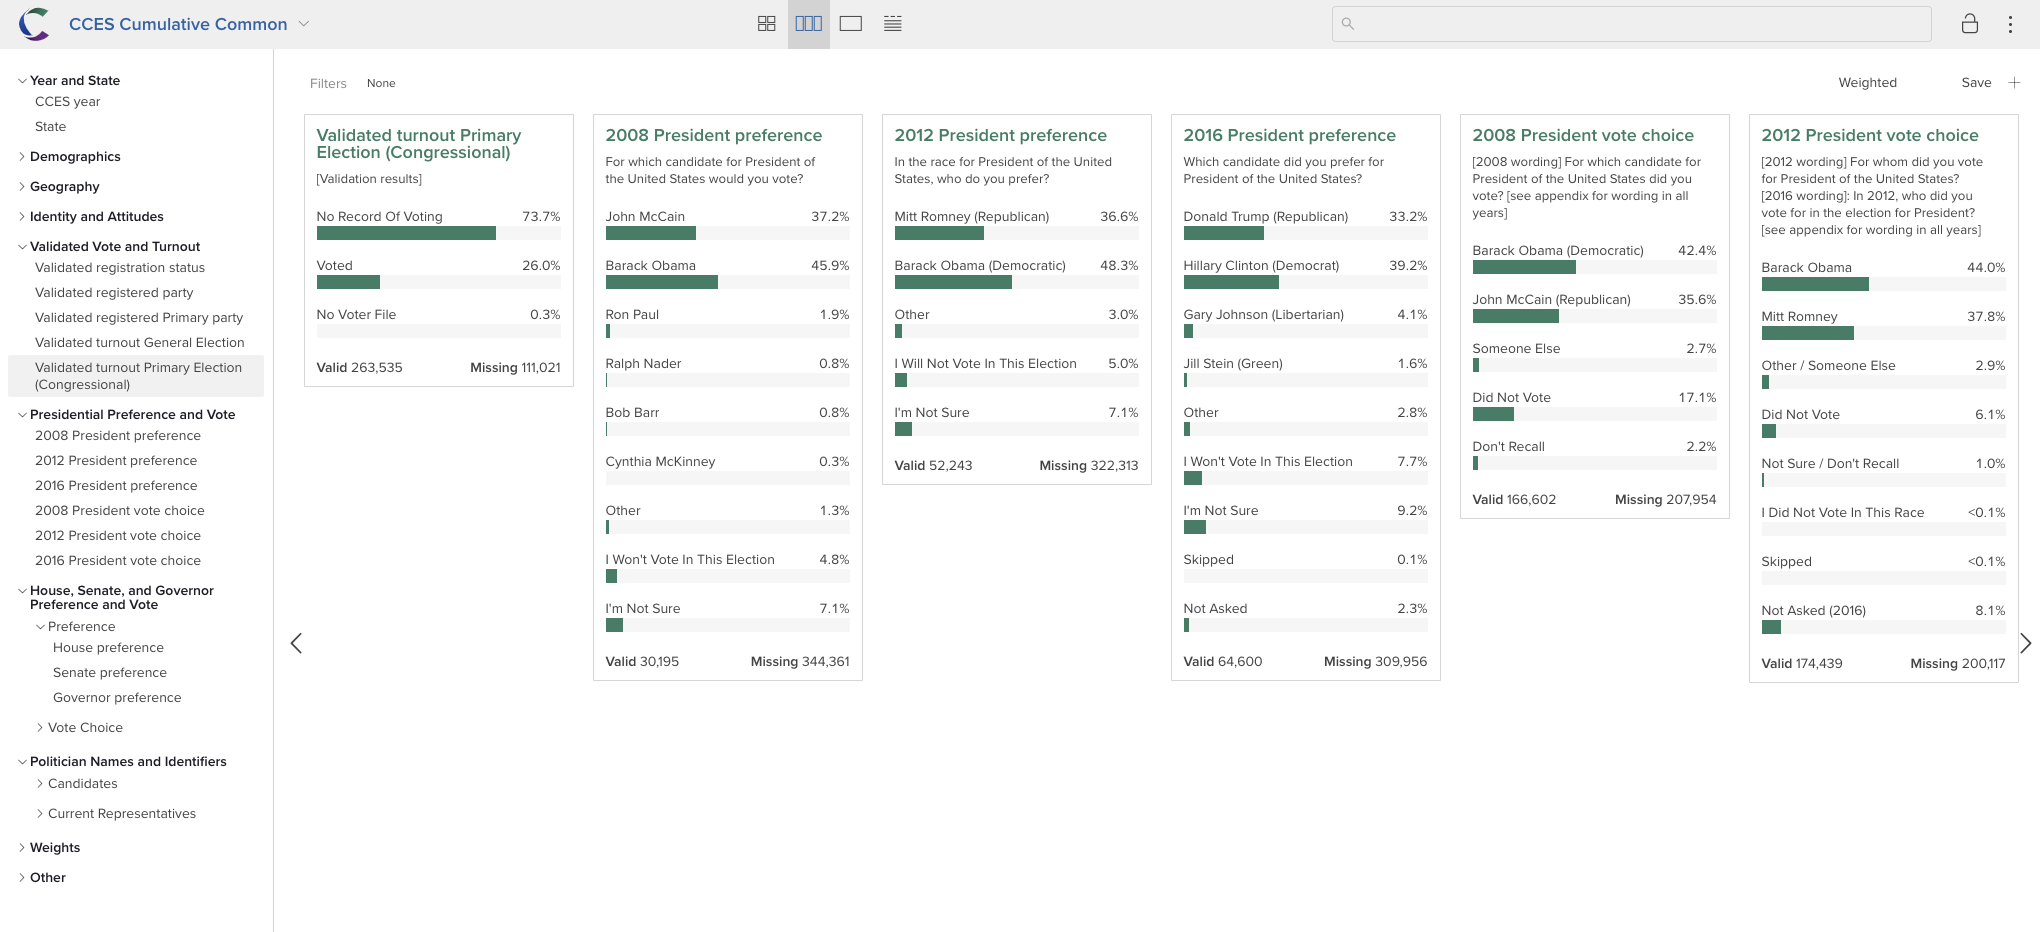
\includegraphics[width=1.05\linewidth]{01_crunch_browse.png}}
\end{figure}

\begin{enumerate}
\def\labelenumi{\arabic{enumi}.}
\setcounter{enumi}{2}
\tightlist
\item
  Analyze: The crunch interface allows Viewers to make cross-tabs and
  bar graphs quickly.\\

  \begin{figure}[H]
  \centering
  \centerline{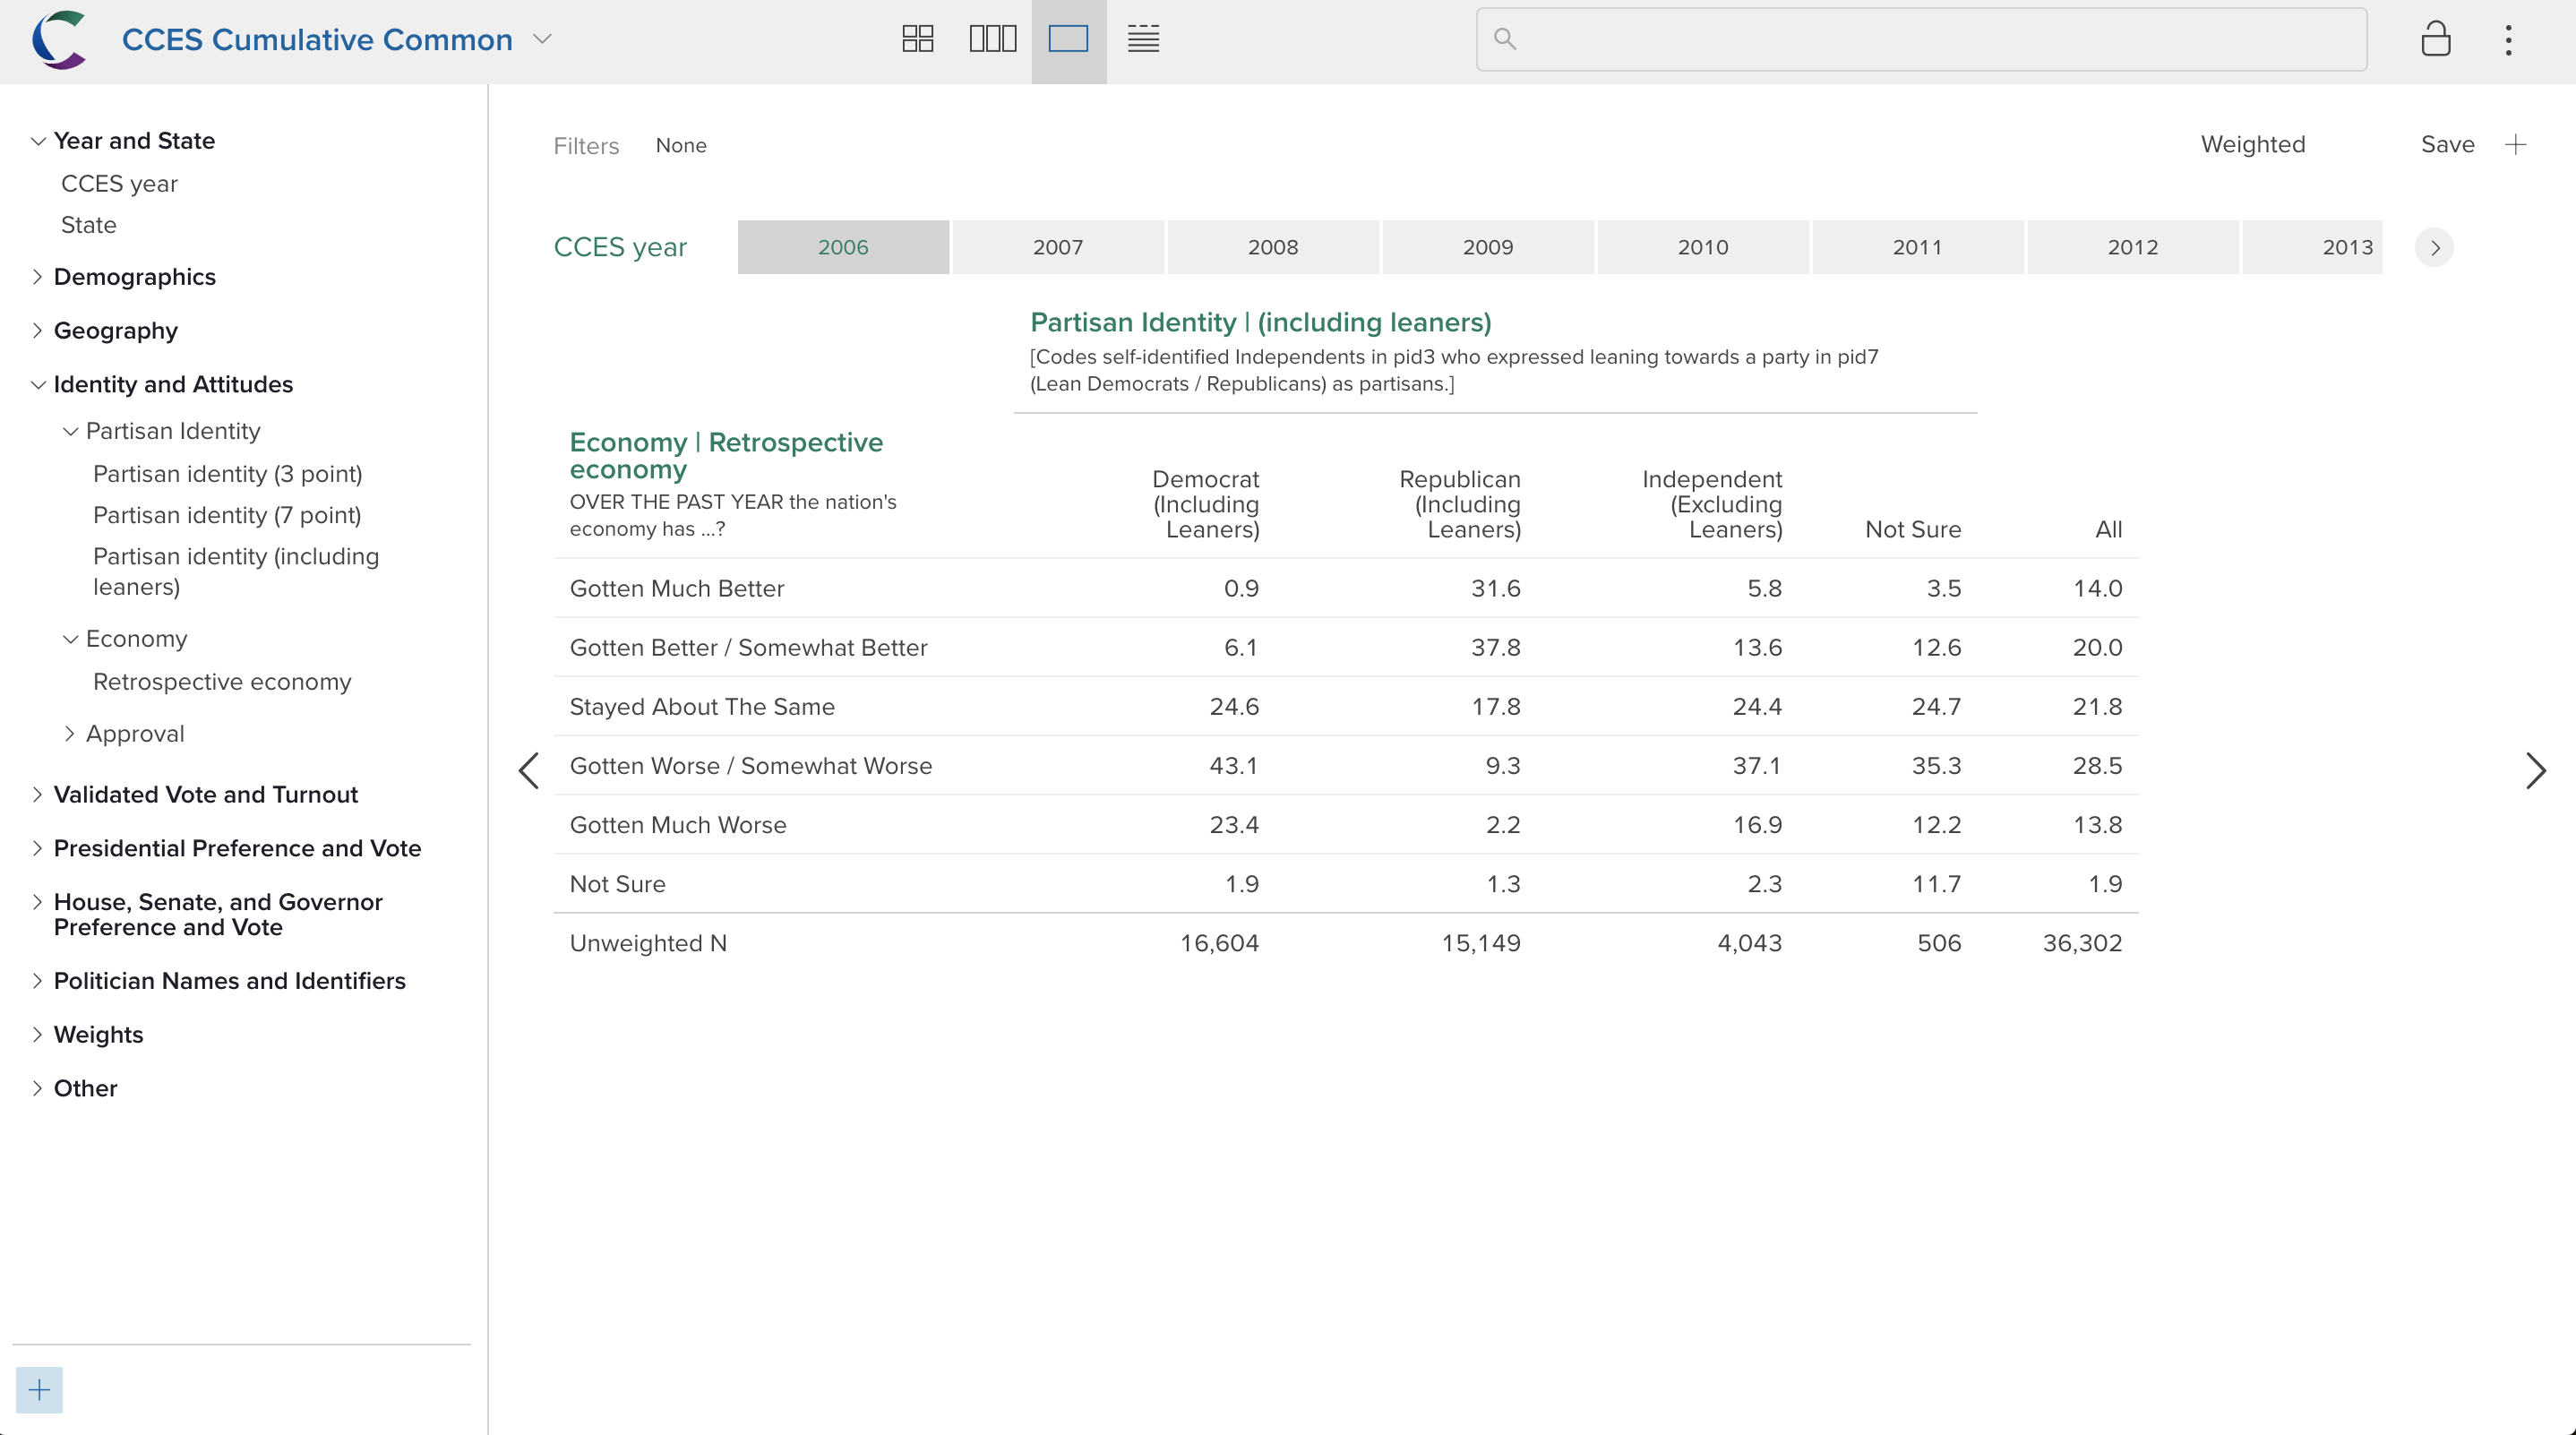
\includegraphics[width=1.05\linewidth]{02_crunch_tab.png}}
  \end{figure}
\end{enumerate}

Crunch datasets can also be manipulated from a R package,
\texttt{crunch} \url{https://github.com/Crunch-io/rcrunch}.

\newpage

\hypertarget{variables}{%
\section{Variables}\label{variables}}

The sections below provide summary more information on each variable.

\begin{itemize}
\tightlist
\item
  The title shows the name as used in the dataset, suitable for coding
  (``alias'' in Crunch terminology). followed by a more descriptive name
  suitable for presentation (``name'' in Crunch terminology).
\item
  Question wordings, where applicable, immediately follow. Otherwise a
  description is provided in square brackets (\texttt{{[}\ \ {]}}). All
  square brackets, both in the description and the response options,
  indicate descriptions that are summaries of what the respondent saw
  rather than the question verbatim.
\item
  A tabulation of response options (or summary statistics for numeric
  variables) follow. Numbers are unweighted counts.
\item
  The ``Years'' bullet lists the years of the CCES in which data on the
  variable is available at all. If a year is not listed, either the
  question was not asked in the year or was not incorporated in the
  creation of this dataset.
\item
  Finally, the ``Limitations'' bullet notes some of the caveats required
  when interpreting this variable. As this dataset is combinations of
  different surveys, some year-specific details on implementation are
  inevitably lost. For example, for all 2016 responses ``Not Asked'' and
  ``Skipped'' are both coded as a \texttt{NA} (missing) to stay
  consistent with past years that did not make that finer distinction.
\end{itemize}

\hypertarget{administration}{%
\section{Administration}\label{administration}}

\hypertarget{year-cces-year}{%
\subsubsection{\texorpdfstring{\texttt{year}: CCES
year}{year: CCES year}}\label{year-cces-year}}

{[}Year of CCES Common Content{]}

\begin{verbatim}
 year     n
 2006 36421
 2007  9999
 2008 32800
 2009 13800
 2010 55400
 2011 20150
 2012 54535
 2013 16400
 2014 56200
 2015 14250
 2016 64600
 2017 18200
 2018 60000
\end{verbatim}

\hypertarget{starttime-start-time}{%
\subsubsection{\texorpdfstring{\texttt{starttime}: Start
time}{starttime: Start time}}\label{starttime-start-time}}

{[}Pre-election wave start time (up to second){]}

\begin{verbatim}
                 Min.               1st Qu.                Median 
"2006-10-07 00:02:34" "2010-10-11 15:40:49" "2013-11-12 10:50:17" 
                 Mean               3rd Qu.                  Max. 
"2013-06-29 00:06:52" "2016-10-10 09:04:56" "2018-11-05 23:27:49" 
\end{verbatim}

\begin{itemize}
\tightlist
\item
  Years: All of 2006-2018
\end{itemize}

\hypertarget{tookpost-took-post-election-wave}{%
\subsubsection{\texorpdfstring{\texttt{tookpost}: Took post-election
wave}{tookpost: Took post-election wave}}\label{tookpost-took-post-election-wave}}

{[}Whether or not the respondent took the post-election wave of the
survey (in even years){]}

\begin{verbatim}
Warning: Factor `tookpost` contains implicit NA, consider using
`forcats::fct_explicit_na`
\end{verbatim}

\begin{verbatim}
                          tookpost      n
 Did Not Take Post-Election Survey  59064
         Took Post-Election Survey 300892
                              <NA>  92799
\end{verbatim}

\begin{itemize}
\tightlist
\item
  Years: 2006, 2008, 2010, 2012, 2014, 2016, 2018 (Post-election wave
  only exists for even years)
\end{itemize}

\hypertarget{weights}{%
\section{Weights}\label{weights}}

\hypertarget{weight-survey-weight-year-specific}{%
\subsubsection{\texorpdfstring{\texttt{weight}: Survey weight
(Year-Specific)}{weight: Survey weight (Year-Specific)}}\label{weight-survey-weight-year-specific}}

{[}weights from pre-election survey of each year{]}

\begin{verbatim}
   Min. 1st Qu.  Median    Mean 3rd Qu.    Max. 
 0.0000  0.4259  0.7281  1.0000  1.1741 15.0006 
\end{verbatim}

\begin{itemize}
\tightlist
\item
  Years: All of 2006-2018
\item
  In even years, they are re-computed after vote validation has been
  computed and those re-computed weights are taken here when available.
  The weights applied to the sample (which is originally drawn from a
  matched sample) are constructed to make each year's respondents' pool
  representative of the national adult population. See the methodology
  section of the
  \href{https://dataverse.harvard.edu/api/access/datafile/3047286}{2016
  Guide} for details.
\item
  Limitations: Only specific to each year. Built off of the entire
  pre-election wave sample, but not necessarily to adjust post-election
  wave respondents. See \texttt{weight\_post}
\end{itemize}

\hypertarget{weight_cumulative-survey-weight-cumulative}{%
\subsubsection{\texorpdfstring{\texttt{weight\_cumulative}: Survey
weight
(Cumulative)}{weight\_cumulative: Survey weight (Cumulative)}}\label{weight_cumulative-survey-weight-cumulative}}

{[}weight variable with simple adjustment: multiplied a constant within
year to make years comparable{]}

\begin{verbatim}
   Min. 1st Qu.  Median    Mean 3rd Qu.    Max.    NA's 
   0.00    0.25    0.48    0.81    0.97   19.40   60000 
\end{verbatim}

\begin{itemize}
\tightlist
\item
  Years: All of 2006-2017
\item
  Limitations: Only a simple transformation of \texttt{weight}.
  Specifically, \texttt{weight\_cumulative} is \texttt{weight} divided
  by the following factor, for a given year.
\end{itemize}

\begin{tabular}{rrr}
\toprule
Year & Observations & Factor\\
\midrule
2006 & 36,421 & 1.38\\
2007 & 9,999 & 0.38\\
2008 & 32,800 & 1.24\\
2009 & 13,800 & 0.52\\
2010 & 55,400 & 2.09\\
\addlinespace
2011 & 20,150 & 0.76\\
2012 & 54,535 & 2.06\\
2013 & 16,400 & 0.62\\
2014 & 56,200 & 2.12\\
2015 & 14,250 & 0.54\\
\addlinespace
2016 & 64,600 & 2.44\\
2017 & 18,200 & 0.69\\
\bottomrule
\end{tabular}

For example, all weights in the 2012 common content are divided by about
2.06, because it has about twice as many observations as the other
datasets.

\hypertarget{weight_post-survey-weight-for-post-election-wave}{%
\subsubsection{\texorpdfstring{\texttt{weight\_post}: Survey weight for
post-election
wave}{weight\_post: Survey weight for post-election wave}}\label{weight_post-survey-weight-for-post-election-wave}}

{[}weight for post-election wave respondents. Only available for some of
the even years.{]}

\begin{verbatim}
   Min. 1st Qu.  Median    Mean 3rd Qu.    Max.    NA's 
   0.00    0.45    0.70    1.00    1.10   15.00  303170 
\end{verbatim}

\begin{itemize}
\tightlist
\item
  Years: 2012, 2016, 2018
\item
  Limitations: Only available for some even years.
\end{itemize}

\hypertarget{geography}{%
\section{Geography}\label{geography}}

A series of variables for the respondent's location

\begin{itemize}
\tightlist
\item
  \texttt{state}: State (FIPS): {[}State (Imputed from input zipcode){]}
\item
  \texttt{st}: State abbreviation (FIPS): {[}State (Imputed from input
  zipcode){]}
\item
  \texttt{dist}: Congressional district number in current Congress:
  {[}Current Congressional District Number (Imputed from input
  zipcode){]}
\item
  \texttt{dist\_up}: Congressional district number for upcoming
  Congress: {[}Upcoming Congressional District Number (Imputed from
  input zipcode){]}
\item
  \texttt{cd}: Congressional district in current Congress: {[}Current
  Congressional District (Imputed from input zipcode){]}
\item
  \texttt{zipcode}: Zipcode of residence: So that we can ask you about
  the news and events in your area, in what zip code do you currently
  reside?
\item
  \texttt{county\_fips}: County of residence: {[}County (Imputed from
  input zipcode){]}
\end{itemize}

\begin{verbatim}
Observations: 452,755
Variables: 7
$ state       <chr> "California", "Pennsylvania", "Texas", "Texas", "T...
$ st          <chr> "CA", "PA", "TX", "TX", "TX", "NY", "NC", "NC", "M...
$ cd          <chr> "CA-2", "PA-5", "TX-16", "TX-19", "TX-6", "NY-28",...
$ dist        <int> 2, 5, 16, 19, 6, 28, 11, 7, 1, 17, 15, 1, 2, 6, 1,...
$ dist_up     <int> 1, 3, 16, 19, 6, 27, 11, 7, 2, 20, 12, 1, 2, 8, 1,...
$ zipcode     <chr> "95969", "16255", "79924", "79423", "76123", "1413...
$ county_fips <chr> "06007", "42031", "48141", "48303", "48439", "3606...
\end{verbatim}

\begin{itemize}
\tightlist
\item
  Years: All of 2006-2018
\item
  Limitations: Some years do not provide the variable relevant to
  \texttt{dist\_up}, in which case the current district (\texttt{dist})
  is assigned automatically. Thus, \texttt{dist\_up} may not reflect,
  for example, district changes in off-cycle redistricting. Only
  residence (not registration) geographies included here; see individual
  years' for registration geographies.
\end{itemize}

\hypertarget{demographics}{%
\section{Demographics}\label{demographics}}

\hypertarget{gender-gender}{%
\subsubsection{\texorpdfstring{\texttt{gender}:
Gender}{gender: Gender}}\label{gender-gender}}

Are you male or female?

\begin{verbatim}
 gender      n
   Male 210102
 Female 242653
\end{verbatim}

\begin{itemize}
\tightlist
\item
  Years: All of 2006-2018
\end{itemize}

\hypertarget{birthyr-year-of-birth}{%
\subsubsection{\texorpdfstring{\texttt{birthyr}: Year of
birth}{birthyr: Year of birth}}\label{birthyr-year-of-birth}}

In what year were you born?

\begin{verbatim}
   Min. 1st Qu.  Median    Mean 3rd Qu.    Max. 
   1900    1950    1961    1963    1977    2000 
\end{verbatim}

\begin{itemize}
\tightlist
\item
  Years: All of 2006-2018
\end{itemize}

\hypertarget{age-age}{%
\subsubsection{\texorpdfstring{\texttt{age}:
Age}{age: Age}}\label{age-age}}

{[}Approximate age computed from the year of survey minus Year of
Birth{]}

\begin{verbatim}
   Min. 1st Qu.  Median    Mean 3rd Qu.    Max. 
  18.00   36.00   51.00   49.61   62.00  109.00 
\end{verbatim}

\begin{itemize}
\tightlist
\item
  Years: All of 2006-2018
\end{itemize}

\hypertarget{educ-education}{%
\subsubsection{\texorpdfstring{\texttt{educ}:
Education}{educ: Education}}\label{educ-education}}

What is the highest level of education you have completed?

\begin{verbatim}
Warning: Factor `educ` contains implicit NA, consider using
`forcats::fct_explicit_na`
\end{verbatim}

\begin{verbatim}
                 educ      n
                No HS  13939
 High School Graduate 125323
         Some College 112290
               2-Year  43606
               4-Year 103011
            Post-Grad  54519
                 <NA>     67
\end{verbatim}

\begin{itemize}
\tightlist
\item
  Years: All of 2006-2018
\end{itemize}

\hypertarget{race-race}{%
\subsubsection{\texorpdfstring{\texttt{race}:
Race}{race: Race}}\label{race-race}}

What racial or ethnic group best describes you?

\begin{verbatim}
            race      n
           White 337793
           Black  49162
        Hispanic  35924
           Asian   9134
 Native American   3543
           Mixed   8919
           Other   7554
  Middle Eastern    726
\end{verbatim}

\begin{itemize}
\tightlist
\item
  Years: All of 2006-2018
\item
  Limitations: The ``Hispanic'' value may undercount self-identified
  Hispanics. See \texttt{hispanic}
\end{itemize}

\hypertarget{hispanic-hispanic}{%
\subsubsection{\texorpdfstring{\texttt{hispanic}:
Hispanic}{hispanic: Hispanic}}\label{hispanic-hispanic}}

Are you of Spanish, Latino, or Hispanic origin or descent? {[}Asked if
response to race is not Hispanic{]}

\begin{verbatim}
Warning: Factor `hispanic` contains implicit NA, consider using
`forcats::fct_explicit_na`
\end{verbatim}

\begin{verbatim}
 hispanic      n
      Yes  11113
       No 321994
     <NA> 119648
\end{verbatim}

\begin{itemize}
\tightlist
\item
  Years: 2010, 2011, 2012, 2013, 2014, 2015, 2016, 2017, 2018
\item
  In years in which this question was fielded, this question supplements
  the \texttt{race} variable by asking does who did \emph{not} respnd
  ``Hipsanic'' in the \texttt{race} question.
\end{itemize}

\hypertarget{faminc-family-income}{%
\subsubsection{\texorpdfstring{\texttt{faminc}: Family
Income}{faminc: Family Income}}\label{faminc-family-income}}

Thinking back over the last year, what was your family's annual income?
{[}Brackets coarsened{]}

\begin{verbatim}
Warning: Factor `faminc` contains implicit NA, consider using
`forcats::fct_explicit_na`
\end{verbatim}

\begin{verbatim}
            faminc     n
     Less than 10k 18780
         10k - 20k 32995
         20k - 30k 46019
         30k - 40k 46728
         40k - 50k 41768
         50k - 60k 40863
         60k - 70k 30063
         70k - 80k 32459
        80k - 100k 37809
       100k - 120k 27566
       120k - 150k 22108
             150k+ 25075
 Prefer not to say 48955
           Skipped    12
              <NA>  1555
\end{verbatim}

\begin{itemize}
\tightlist
\item
  Years: All of 2006-2018
\item
  Limitations: The income brackets provided changed slightly over time.
  The brackets in this cumulative dataset coarsens some brackets, with
  loss of some granularity. In particular, from 2011-2016, respondents
  answering ``over 150k'' were asked in a follow-up question when the
  respondent initially selected ``over 150k''. These are top-coded and
  only labelled as ``over 150k.''
\item
  The 2009 CCES did not have an option for 60-70k.
\end{itemize}

\hypertarget{marstat-marital-status}{%
\subsubsection{\texorpdfstring{\texttt{marstat}: Marital
Status}{marstat: Marital Status}}\label{marstat-marital-status}}

What is your marital status?

\begin{verbatim}
Warning: Factor `marstat` contains implicit NA, consider using
`forcats::fct_explicit_na`
\end{verbatim}

\begin{verbatim}
              marstat      n
              Married 250629
            Separated   7606
             Divorced  49651
              Widowed  21287
               Single 101416
 Domestic Partnership  20611
                 <NA>   1555
\end{verbatim}

\begin{itemize}
\tightlist
\item
  Years: All of 2006-2018
\end{itemize}

\newpage

\hypertarget{validations}{%
\section{Validations}\label{validations}}

Observations in even years include (or will include) indicators for
validated voting, which means that YouGov has matched survey
respondents' personal identifiable information to public voter files,
which in turn officially record whether a person has voted or not.
Validation is often completed in the summer following the election; 2018
validation data is not available as of March. For more information, see
\href{https://doi.org/10.1093/pan/mps023}{Ansolabehere and Hersh
(2012)}.

\hypertarget{vv_regstatus-validated-registration-status}{%
\subsubsection{\texorpdfstring{\texttt{vv\_regstatus}: Validated
registration
status}{vv\_regstatus: Validated registration status}}\label{vv_regstatus-validated-registration-status}}

{[}Validation results. Missing if validation was not conducted in the
year. Categories are aggregated. Both Matched-not registered and
unmatched are labeled as a no record.{]}

\begin{verbatim}
Warning: Factor `vv_regstatus` contains implicit NA, consider using
`forcats::fct_explicit_na`
\end{verbatim}

\begin{verbatim}
              vv_regstatus      n
                    Active 178356
 No Record Of Registration  61861
              Unregistered  13826
                   Dropped   5294
                  Inactive   3047
      Multiple Appearances   1151
                      <NA> 189220
\end{verbatim}

\begin{itemize}
\tightlist
\item
  Years: 2008, 2010, 2012, 2014, 2016
\item
  Limitations: Collapses some response options
\end{itemize}

\hypertarget{vv_party_gen-validated-registered-party}{%
\subsubsection{\texorpdfstring{\texttt{vv\_party\_gen}: Validated
registered
party}{vv\_party\_gen: Validated registered party}}\label{vv_party_gen-validated-registered-party}}

{[}Validation results. Only available for some staets and years{]}

\begin{verbatim}
Warning: Factor `vv_party_gen` contains implicit NA, consider using
`forcats::fct_explicit_na`
\end{verbatim}

\begin{verbatim}
                    vv_party_gen      n
 No Record Of Party Registration  60890
                         Unknown  51379
                Democratic Party  27058
                Republican Party  21522
            No Party Affiliation   9835
               Declined To State   1579
                           Other   1286
               Independent Party   1176
              Liberatarian Party    376
                     Green Party    194
              Constitution Party     27
                    Reform Party      9
                 Socialist Party      3
                             Cns      1
                            <NA> 277420
\end{verbatim}

\begin{itemize}
\tightlist
\item
  Years: 2012, 2014, 2016
\item
  Limitations: Not available for some even years
\end{itemize}

\hypertarget{vv_party_prm-validated-registered-primary-party}{%
\subsubsection{\texorpdfstring{\texttt{vv\_party\_prm}: Validated
registered Primary
party}{vv\_party\_prm: Validated registered Primary party}}\label{vv_party_prm-validated-registered-primary-party}}

{[}Validation results. Only available for some staets and years{]}

\begin{verbatim}
Warning: Factor `vv_party_prm` contains implicit NA, consider using
`forcats::fct_explicit_na`
\end{verbatim}

\begin{verbatim}
                    vv_party_prm      n
 No Record Of Party Registration 157120
                Republican Party  10010
                Democratic Party   8202
                           Other      3
                            <NA> 277420
\end{verbatim}

\begin{itemize}
\tightlist
\item
  Years: 2012, 2014, 2016
\item
  Limitations: Not available for some even years
\end{itemize}

\hypertarget{turnout}{%
\subsection{Turnout}\label{turnout}}

\hypertarget{vv_turnout_gvm-validated-turnout-general-election}{%
\subsubsection{\texorpdfstring{\texttt{vv\_turnout\_gvm}: Validated
turnout General
Election}{vv\_turnout\_gvm: Validated turnout General Election}}\label{vv_turnout_gvm-validated-turnout-general-election}}

{[}Validation results. All vote methods (polling, mail, early, unknown,
etc..) are aggregated as a vote.{]}

\begin{verbatim}
Warning: Factor `vv_turnout_gvm` contains implicit NA, consider using
`forcats::fct_explicit_na`
\end{verbatim}

\begin{verbatim}
      vv_turnout_gvm      n
               Voted 169204
 No Record Of Voting 129019
       No Voter File   1733
                <NA> 152799
\end{verbatim}

\begin{itemize}
\tightlist
\item
  Years: 2006, 2008, 2010, 2012, 2014, 2016
\item
  Limitations: Collapses most response options. For example, the
  particular voting method is collapsed into one category, even though
  \texttt{gvm} stands for General Election voting \emph{method}. Also,
  the result of not matching to a voter file is collapsed with the
  result of matching to a voter file and having no indication of turning
  out to vote. The distinction is unclear in earlier years, and is thus
  collapsed for all years here. For finer distinctions, see the
  individual year's CCES.
\end{itemize}

\hypertarget{vv_turnout_pvm-validated-turnout-primary-election-congressional}{%
\subsubsection{\texorpdfstring{\texttt{vv\_turnout\_pvm}: Validated
turnout Primary Election
(Congressional)}{vv\_turnout\_pvm: Validated turnout Primary Election (Congressional)}}\label{vv_turnout_pvm-validated-turnout-primary-election-congressional}}

{[}Validation results{]}

\begin{verbatim}
Warning: Factor `vv_turnout_pvm` contains implicit NA, consider using
`forcats::fct_explicit_na`
\end{verbatim}

\begin{verbatim}
      vv_turnout_pvm      n
 No Record Of Voting 185927
               Voted  76245
       No Voter File   1363
                <NA> 189220
\end{verbatim}

\begin{itemize}
\tightlist
\item
  Years: 2008, 2010, 2012, 2014, 2016
\item
  Limitations: See \texttt{vv\_turnout\_gvm}
\end{itemize}

\newpage

\hypertarget{identity-and-attitudes}{%
\section{Identity and Attitudes}\label{identity-and-attitudes}}

\hypertarget{partisan-identity}{%
\subsection{Partisan Identity}\label{partisan-identity}}

\hypertarget{pid3-partisan-identity-3-point}{%
\subsubsection{\texorpdfstring{\texttt{pid3}: Partisan identity (3
point)}{pid3: Partisan identity (3 point)}}\label{pid3-partisan-identity-3-point}}

Generally speaking, do you think of yourself as a \ldots{}?

\begin{verbatim}
Warning: Factor `pid3` contains implicit NA, consider using
`forcats::fct_explicit_na`
\end{verbatim}

\begin{verbatim}
        pid3      n
    Democrat 160637
  Republican 118907
 Independent 126270
       Other  17975
    Not Sure  20012
        <NA>   8954
\end{verbatim}

\begin{itemize}
\tightlist
\item
  Years: All of 2006-2018
\item
  Limitations: Response options offer slightly by year. For example, the
  \texttt{Not\ Sure} option is not a response option in years 2006 and
  2010. Open-text responses not included. 2010 values are from the
  post-election wave.
\end{itemize}

\hypertarget{pid7-partisan-identity-7-point}{%
\subsubsection{\texorpdfstring{\texttt{pid7}: Partisan identity (7
point)}{pid7: Partisan identity (7 point)}}\label{pid7-partisan-identity-7-point}}

{[}Based on branching from Partisan Identity question{]}

\begin{verbatim}
Warning: Factor `pid7` contains implicit NA, consider using
`forcats::fct_explicit_na`
\end{verbatim}

\begin{verbatim}
                       pid7      n
            Strong Democrat 107733
   Not Very Strong Democrat  54838
              Lean Democrat  45411
                Independent  60946
            Lean Republican  47739
 Not Very Strong Republican  43810
          Strong Republican  75782
                   Not Sure  13480
                       <NA>   3016
\end{verbatim}

\begin{itemize}
\tightlist
\item
  Years: All of 2006-2018
\item
  Limitations: See \texttt{pid3}
\end{itemize}

\hypertarget{pid3_leaner-partisan-identity-including-leaners}{%
\subsubsection{\texorpdfstring{\texttt{pid3\_leaner}: Partisan identity
(including
leaners)}{pid3\_leaner: Partisan identity (including leaners)}}\label{pid3_leaner-partisan-identity-including-leaners}}

{[}Codes self-identified Independents in pid3 who expressed leaning
towards a party in pid7 (Lean Democrats / Republicans) as partisans.{]}

\begin{verbatim}
Warning: Factor `pid3_leaner` contains implicit NA, consider using
`forcats::fct_explicit_na`
\end{verbatim}

\begin{verbatim}
                     pid3_leaner      n
    Democrat (Including Leaners) 207982
  Republican (Including Leaners) 167331
 Independent (Excluding Leaners)  60946
                        Not Sure  13480
                            <NA>   3016
\end{verbatim}

\begin{itemize}
\tightlist
\item
  Years: All of 2006-2018
\item
  Limitations: See \texttt{pid3}
\end{itemize}

\hypertarget{ideo5-ideology-5-point}{%
\subsubsection{\texorpdfstring{\texttt{ideo5}: Ideology (5
point)}{ideo5: Ideology (5 point)}}\label{ideo5-ideology-5-point}}

In general, how would you describe your own political viewpoint?

\begin{verbatim}
Warning: Factor `ideo5` contains implicit NA, consider using
`forcats::fct_explicit_na`
\end{verbatim}

\begin{verbatim}
             ideo5      n
      Very Liberal  40142
           Liberal  79591
          Moderate 141633
      Conservative 105268
 Very Conservative  52243
          Not Sure  32104
              <NA>   1774
\end{verbatim}

\begin{itemize}
\tightlist
\item
  Years: All of 2006-2018
\end{itemize}

\hypertarget{economy}{%
\subsection{Economy}\label{economy}}

\hypertarget{economy_retro-retrospective-economy}{%
\subsubsection{\texorpdfstring{\texttt{economy\_retro}: Retrospective
economy}{economy\_retro: Retrospective economy}}\label{economy_retro-retrospective-economy}}

OVER THE PAST YEAR the nation's economy has \ldots{}?

\begin{verbatim}
Warning: Factor `economy_retro` contains implicit NA, consider using
`forcats::fct_explicit_na`
\end{verbatim}

\begin{verbatim}
                   economy_retro      n
              Gotten Much Better  29702
 Gotten Better / Somewhat Better 100766
           Stayed About The Same 118229
   Gotten Worse / Somewhat Worse 114965
               Gotten Much Worse  77949
                        Not Sure  10294
                            <NA>    850
\end{verbatim}

\begin{itemize}
\tightlist
\item
  Years: All of 2006-2018
\item
  Limitations: Response options varies by year. Some are collapsed into
  one category (e.g. \texttt{Gotten\ Better}, presented in some years,
  and \texttt{Gotten\ Somewhat\ Better}, presented in other years, are
  collapsed into \texttt{Gotten\ Better\ /\ Somewhat\ Better}). Some are
  left as is. For example, \texttt{Not\ Sure} was not an option in 2009.
\end{itemize}

\hypertarget{news-interest}{%
\subsection{News Interest}\label{news-interest}}

\hypertarget{newsint-news-interest}{%
\subsubsection{\texorpdfstring{\texttt{newsint}: News
Interest}{newsint: News Interest}}\label{newsint-news-interest}}

Some people seem to follow what's going on in government and public
affairs most of the time, whether there's an election going on or not.
Others aren't that interested. Would you say you follow what's going on
in government and public affairs ..

\begin{verbatim}
Warning: Factor `newsint` contains implicit NA, consider using
`forcats::fct_explicit_na`
\end{verbatim}

\begin{verbatim}
           newsint      n
  Most Of The Time 225200
  Some Of The Time 105337
 Only Now And Then  50141
     Hardly At All  24621
        Don't Know  10449
              <NA>  37007
\end{verbatim}

\begin{itemize}
\tightlist
\item
  Years: 2007, 2008, 2009, 2010, 2011, 2012, 2013, 2014, 2015, 2016,
  2017, 2018
\item
  Limitations: Not asked in 2006. Similar questions about watching TV
  news was asked in 2006.
\end{itemize}

\hypertarget{approval}{%
\subsection{Approval}\label{approval}}

\hypertarget{approval_pres-president-approval}{%
\subsubsection{\texorpdfstring{\texttt{approval\_pres}: President
approval}{approval\_pres: President approval}}\label{approval_pres-president-approval}}

Do you approve of the way each is doing their job\ldots{} {[}Pipe
Incumbent President{]}

\begin{verbatim}
Warning: Factor `approval_pres` contains implicit NA, consider using
`forcats::fct_explicit_na`
\end{verbatim}

\begin{verbatim}
                  approval_pres      n
               Strongly Approve  92872
               Somewhat Approve 104677
            Somewhat Disapprove  47005
            Strongly Disapprove 194516
                       Not Sure  12507
 Neither Approve Nor Disapprove    443
                           <NA>    735
\end{verbatim}

\begin{itemize}
\tightlist
\item
  Years: All of 2006-2018
\item
  Limitations: \texttt{Neither\ approve\ nor\ disapprove} only included
  in 2007.
\item
  This question is asked in a grid format, along with Governors,
  Congress, and Courts.
\end{itemize}

\hypertarget{approval_rep-house-representative-approval}{%
\subsubsection{\texorpdfstring{\texttt{approval\_rep}: House
Representative
approval}{approval\_rep: House Representative approval}}\label{approval_rep-house-representative-approval}}

Do you approve of the way each is doing their job\ldots{} {[}Pipe
Incumbent Representative's Name{]}

\begin{verbatim}
Warning: Factor `approval_rep` contains implicit NA, consider using
`forcats::fct_explicit_na`
\end{verbatim}

\begin{verbatim}
                     approval_rep      n
                 Strongly Approve  65102
       Approve / Somewhat Approve 142503
 Disapprove / Somewhat Disapprove  79595
              Strongly Disapprove  70663
           Never Heard / Not Sure  85772
   Neither Approve Nor Disapprove   1798
                             <NA>   7322
\end{verbatim}

\begin{itemize}
\tightlist
\item
  Years: All of 2006-2018
\item
  Limitations: \texttt{Neither\ approve\ nor\ disapprove} only included
  in 2007.
\item
  This question is asked in a grid format, along with Senators
  (\texttt{approval\_sen1}, \texttt{approval\_sen2}).
\item
  To see who {[}Representative{]} refers to for a particular respondent,
  see \texttt{rep\_inc} (incumbent identifier in \texttt{rep\_icpsr})
\end{itemize}

\hypertarget{approval_sen1-senator-1-approval}{%
\subsubsection{\texorpdfstring{\texttt{approval\_sen1}: Senator 1
approval}{approval\_sen1: Senator 1 approval}}\label{approval_sen1-senator-1-approval}}

Do you approve of the way each is doing their job\ldots{} {[}Pipe
Incumbent Senator 1's Name{]}

\begin{verbatim}
Warning: Factor `approval_sen1` contains implicit NA, consider using
`forcats::fct_explicit_na`
\end{verbatim}

\begin{verbatim}
                    approval_sen1      n
                 Strongly Approve  58761
       Approve / Somewhat Approve 144415
 Disapprove / Somewhat Disapprove  90846
              Strongly Disapprove  89017
           Never Heard / Not Sure  63783
   Neither Approve Nor Disapprove   1413
                             <NA>   4520
\end{verbatim}

\begin{itemize}
\tightlist
\item
  Years: All of 2006-2018
\item
  Limitations: : Response options varies by year. Some are collapsed
  into one category (e.g. \texttt{Approve}, presented in some years, and
  \texttt{Somewhat\ Approve}, presented in other years, are collapsed
  into \texttt{Approve\ /\ Somewhat\ Approve}).
  \texttt{Neither\ approve\ nor\ disapprove} only included in 2007.
\item
  To see who {[}Senator 1{]} refers to for a particular respondent, see
  \texttt{sen1\_inc} (incumbent identifier in \texttt{sen1\_icpsr})
\end{itemize}

\hypertarget{approval_sen2-senator-2-approval}{%
\subsubsection{\texorpdfstring{\texttt{approval\_sen2}: Senator 2
approval}{approval\_sen2: Senator 2 approval}}\label{approval_sen2-senator-2-approval}}

Do you approve of the way each is doing their job\ldots{} {[}Pipe
Incumbent Senator 2's Name{]}

\begin{verbatim}
Warning: Factor `approval_sen2` contains implicit NA, consider using
`forcats::fct_explicit_na`
\end{verbatim}

\begin{verbatim}
                    approval_sen2      n
                 Strongly Approve  63135
       Approve / Somewhat Approve 139337
 Disapprove / Somewhat Disapprove  88539
              Strongly Disapprove  89232
           Never Heard / Not Sure  66076
   Neither Approve Nor Disapprove   1158
                             <NA>   5278
\end{verbatim}

\begin{itemize}
\tightlist
\item
  See \texttt{approval\_sen2}
\end{itemize}

\hypertarget{approval_gov-governor-approval}{%
\subsubsection{\texorpdfstring{\texttt{approval\_gov}: Governor
approval}{approval\_gov: Governor approval}}\label{approval_gov-governor-approval}}

Do you approve of the way each is doing their job\ldots{} Governor of
{[}Pipe State{]}

\begin{verbatim}
Warning: Factor `approval_gov` contains implicit NA, consider using
`forcats::fct_explicit_na`
\end{verbatim}

\begin{verbatim}
                   approval_gov      n
               Strongly Approve  67404
               Somewhat Approve 139940
            Somewhat Disapprove  84271
            Strongly Disapprove 117282
                       Not Sure  40318
 Neither Approve Nor Disapprove   1414
                           <NA>   2126
\end{verbatim}

\begin{itemize}
\tightlist
\item
  Years: All of 2006-2018
\item
  Limitations: See \texttt{approval\_pres}
\item
  To see who the Governor refers to for a particular respondent, see
  \texttt{gov\_inc} (incumbent identifier in \texttt{gov\_fec}, if
  applicable).
\end{itemize}

\newpage

\hypertarget{presidential-vote}{%
\section{Presidential Vote}\label{presidential-vote}}

\begin{tcolorbox}[title={A note on \texttt{intent} and \texttt{voted}}]
In this dataset we make the distinction between "intent" / "preference" vs. "voted" / "vote choice". "Intent" (or "preference") refers to the response to the prospective question of the sort "who would you vote for?" in the \emph{pre-election} wave. "Vote choice" refers to the response to the retrospective question of the sort "in the election this November, who did you vote for?" Response to the vote choice questions coalesces both \emph{post-election} wave responses (the bulk of the responses) and pre-election respondents who reported having already voted early. 
\end{tcolorbox}

\hypertarget{intent_pres_08-2008-president-preference-before-voting}{%
\subsubsection{\texorpdfstring{\texttt{intent\_pres\_08}: 2008 President
preference (before
voting)}{intent\_pres\_08: 2008 President preference (before voting)}}\label{intent_pres_08-2008-president-preference-before-voting}}

For which candidate for President of the United States would you vote?

\begin{verbatim}
Warning: Factor `intent_pres_08` contains implicit NA, consider using
`forcats::fct_explicit_na`
\end{verbatim}

\begin{verbatim}
                intent_pres_08      n
                   John McCain  13322
                  Barack Obama  12897
                      Ron Paul    535
                   Ralph Nader    209
                      Bob Barr    258
              Cynthia McKinney     74
                         Other    352
 I Won't Vote In This Election    851
                  I'm Not Sure   1697
                          <NA> 422560
\end{verbatim}

\begin{itemize}
\tightlist
\item
  Years: 2008
\end{itemize}

\hypertarget{intent_pres_12-2012-president-preference-before-voting}{%
\subsubsection{\texorpdfstring{\texttt{intent\_pres\_12}: 2012 President
preference (before
voting)}{intent\_pres\_12: 2012 President preference (before voting)}}\label{intent_pres_12-2012-president-preference-before-voting}}

In the race for President of the United States, who do you prefer?

\begin{verbatim}
Warning: Factor `intent_pres_12` contains implicit NA, consider using
`forcats::fct_explicit_na`
\end{verbatim}

\begin{verbatim}
                   intent_pres_12      n
         Mitt Romney (Republican)  20738
        Barack Obama (Democratic)  24401
                            Other   1781
 I Will Not Vote In This Election   1467
                     I'm Not Sure   3856
                             <NA> 400512
\end{verbatim}

\begin{itemize}
\tightlist
\item
  Years: 2012
\end{itemize}

\hypertarget{intent_pres_16-2016-president-preference-before-voting}{%
\subsubsection{\texorpdfstring{\texttt{intent\_pres\_16}: 2016 President
preference (before
voting)}{intent\_pres\_16: 2016 President preference (before voting)}}\label{intent_pres_16-2016-president-preference-before-voting}}

Which candidate did you prefer for President of the United States?

\begin{verbatim}
Warning: Factor `intent_pres_16` contains implicit NA, consider using
`forcats::fct_explicit_na`
\end{verbatim}

\begin{verbatim}
                intent_pres_16      n
     Donald Trump (Republican)  19227
    Hillary Clinton (Democrat)  27502
    Gary Johnson (Libertarian)   3145
            Jill Stein (Green)   1400
                         Other   1880
 I Won't Vote In This Election   3312
                  I'm Not Sure   6536
                          <NA> 389753
\end{verbatim}

\begin{itemize}
\tightlist
\item
  Years: 2016
\end{itemize}

\hypertarget{voted_pres_08-2008-president-vote-choice-after-voting}{%
\subsubsection{\texorpdfstring{\texttt{voted\_pres\_08}: 2008 President
vote choice (after
voting)}{voted\_pres\_08: 2008 President vote choice (after voting)}}\label{voted_pres_08-2008-president-vote-choice-after-voting}}

2008: For which candidate for President of the United States did you
vote? {[}see guide for wording in all years{]}

\begin{verbatim}
Warning: Factor `voted_pres_08` contains implicit NA, consider using
`forcats::fct_explicit_na`
\end{verbatim}

\begin{verbatim}
             voted_pres_08      n
 Barack Obama (Democratic)  73986
  John McCain (Republican)  68398
              Someone Else   4204
              Did Not Vote  18227
              Don't Recall   1787
                      <NA> 286153
\end{verbatim}

\begin{itemize}
\tightlist
\item
  Years: 2008, 2009, 2010, 2011, 2012
\item
  Limitations: Response options offer slightly by year; some are
  collapsed into one.
\end{itemize}

\hypertarget{voted_pres_12-2012-president-vote-choice-after-voting}{%
\subsubsection{\texorpdfstring{\texttt{voted\_pres\_12}: 2012 President
vote choice (after
voting)}{voted\_pres\_12: 2012 President vote choice (after voting)}}\label{voted_pres_12-2012-president-vote-choice-after-voting}}

2012: For whom did you vote for President of the United States? 2016: In
2012, who did you vote for in the election for President? {[}see guide
for wording in all years{]}

\begin{verbatim}
Warning: Factor `voted_pres_12` contains implicit NA, consider using
`forcats::fct_explicit_na`
\end{verbatim}

\begin{verbatim}
               voted_pres_12      n
                Barack Obama  82681
                 Mitt Romney  64956
        Other / Someone Else   5890
                Did Not Vote   2758
     Not Sure / Don't Recall   1990
 I Did Not Vote In This Race     81
                        <NA> 294399
\end{verbatim}

\begin{itemize}
\tightlist
\item
  Years: 2012, 2013, 2014, 2015, 2016
\item
  Limitations: Response options offer slightly by year; some are
  collapsed into one.
\item
  This variable coalesces two variables: Either the response to the
  early vote question in the pre-election wave if the respondent
  indicates they have already voted, or if not, the response in the
  post-election wave.
\end{itemize}

\hypertarget{voted_pres_16-2016-president-vote-choice-after-voting}{%
\subsubsection{\texorpdfstring{\texttt{voted\_pres\_16}: 2016 President
vote choice (after
voting)}{voted\_pres\_16: 2016 President vote choice (after voting)}}\label{voted_pres_16-2016-president-vote-choice-after-voting}}

2017: In the election for U.S. President, who did you vote for? {[}If
reported voting{]} 2016: For whom did you vote for President of the
United States? {[}Post-election{]}

\begin{verbatim}
Warning: Factor `voted_pres_16` contains implicit NA, consider using
`forcats::fct_explicit_na`
\end{verbatim}

\begin{verbatim}
           voted_pres_16      n
            Donald Trump  43891
          Hilary Clinton  51342
    Other / Someone Else  10091
            Did Not Vote    627
 Not Sure / Don't Recall    527
                    <NA> 346277
\end{verbatim}

\begin{itemize}
\tightlist
\item
  Years: 2016, 2017, 2018
\item
  This variable coalesces two variables in the CCES: Either the response
  to the early vote question in the pre-election wave if the respondent
  indicates they have already voted, or if not, the response in the
  post-election wave.
\end{itemize}

\hypertarget{house-senate-and-governor-voting}{%
\section{House, Senate and Governor
Voting}\label{house-senate-and-governor-voting}}

\hypertarget{preference}{%
\subsection{Preference}\label{preference}}

\hypertarget{intent_rep-house-preference-before-voting}{%
\subsubsection{\texorpdfstring{\texttt{intent\_rep}: House preference
(before
voting)}{intent\_rep: House preference (before voting)}}\label{intent_rep-house-preference-before-voting}}

In the general election for U.S. House of Representatives in your area,
who do you prefer? See \texttt{intent\_rep\_party} for party
affiliation.

\begin{verbatim}
Warning: Factor `intent_rep` contains implicit NA, consider using
`forcats::fct_explicit_na`
\end{verbatim}

\begin{verbatim}
                           intent_rep      n
             [Democrat / Candidate 1] 128231
           [Republican / Candidate 2] 115292
                [Other / Candidate 3]   4401
   $HouseCand4Name ($HouseCand4Party)     37
                                Other   2259
                         I'm Not Sure  70460
                               No One  19235
   $HouseCand5Name ($HouseCand5Party)     23
        I Won't Vote In This Election   2269
   $HouseCand6Name ($HouseCand6Party)     41
   $HouseCand7Name ($HouseCand7Party)     20
   $HouseCand8Name ($HouseCand8Party)     14
   $HouseCand9Name ($HouseCand9Party)      1
 $HouseCand10Name ($HouseCand10Party)      1
 $HouseCand11Name ($HouseCand11Party)      3
                                 <NA> 110468
\end{verbatim}

\begin{itemize}
\tightlist
\item
  Years: 2006, 2008, 2010, 2012, 2014, 2016, 2018
\item
  Limitations: Only available for even years. The third party candidate
  not specified for early years. The fourth candidate and onward not
  shown for most years. Response options differ by year.
\item
  Note that it is not always the case that 1 is a Democrat and 2 is a
  Republican. When two Democrats are on the general ballot (e.g.~in
  top-two primary states like California), both candidates are
  Democrats. Use \texttt{intent\_rep\_party} for party affiliation.
\item
  Note that for each respondent, a name (and party affiliation) is shown
  in place of the square bracket values. To see the candidate chosen,
  see \texttt{intent\_rep\_chosen}.
  \texttt{{[}Other\ /\ Candidate\ 3{]}} refers to the third option
  presented, whereas \texttt{Other} refers to the unnamed choice after
  all numbered candidates.
\end{itemize}

\hypertarget{intent_sen-senate-preference-before-voting}{%
\subsubsection{\texorpdfstring{\texttt{intent\_sen}: Senate preference
(before
voting)}{intent\_sen: Senate preference (before voting)}}\label{intent_sen-senate-preference-before-voting}}

In the race for U.S. Senator in your state, who do you prefer? See
\texttt{intent\_sen\_party} for party affiliation.

\begin{verbatim}
Warning: Factor `intent_sen` contains implicit NA, consider using
`forcats::fct_explicit_na`
\end{verbatim}

\begin{verbatim}
                     intent_sen      n
       [Democrat / Candidate 1]  97220
     [Republican / Candidate 2]  82433
          [Other / Candidate 3]   4477
 $SenCand4Name ($SenCand4Party)     19
                          Other   1713
                   I'm Not Sure  38112
                         No One  12419
  I Won't Vote In This Election   1145
                           <NA> 215217
\end{verbatim}

\begin{itemize}
\tightlist
\item
  Years: 2006, 2008, 2010, 2012, 2014, 2016, 2018
\item
  Limitations: See \texttt{intente\_rep}. When both senate seats are up
  for re-election in the same year, only responses to the first senate
  seat is incorporated. For the second senate seat, see individual
  year's CCES.
\end{itemize}

\hypertarget{intent_gov-governor-preference-before-voting}{%
\subsubsection{\texorpdfstring{\texttt{intent\_gov}: Governor preference
(before
voting)}{intent\_gov: Governor preference (before voting)}}\label{intent_gov-governor-preference-before-voting}}

In the race for Governor in your state, who do you prefer? See
\texttt{intent\_gov\_party} for party affiliation.

\begin{verbatim}
Warning: Factor `intent_gov` contains implicit NA, consider using
`forcats::fct_explicit_na`
\end{verbatim}

\begin{verbatim}
                    intent_gov      n
      [Democrat / Candidate 1]  74561
    [Republican / Candidate 2]  66292
         [Other / Candidate 3]   4055
                         Other   1390
                  I'm Not Sure  24296
                        No One   7991
 I Won't Vote In This Election    466
                          <NA> 273704
\end{verbatim}

\begin{itemize}
\tightlist
\item
  Years: 2006, 2008, 2010, 2012, 2014, 2016, 2018
\item
  Limitations: See \texttt{intente\_rep}. For governor elections in odd
  years, see individual year's CCES.
\end{itemize}

\hypertarget{vote-choice}{%
\subsection{Vote Choice}\label{vote-choice}}

\hypertarget{voted_rep-house-vote-choice-after-voting}{%
\subsubsection{\texorpdfstring{\texttt{voted\_rep}: House vote choice
(after
voting)}{voted\_rep: House vote choice (after voting)}}\label{voted_rep-house-vote-choice-after-voting}}

For whom did you vote for U.S. House? See \texttt{voted\_rep\_party} for
party affiliation.

\begin{verbatim}
Warning: Factor `voted_rep` contains implicit NA, consider using
`forcats::fct_explicit_na`
\end{verbatim}

\begin{verbatim}
                            voted_rep      n
             [Democrat / Candidate 1] 115799
           [Republican / Candidate 2] 109342
                [Other / Candidate 3]   2786
   $HouseCand4Name ($HouseCand4Party)     27
                                Other   3124
          I Did Not Vote In This Race  12539
   $HouseCand5Name ($HouseCand5Party)     24
                             Not Sure   4493
   $HouseCand6Name ($HouseCand6Party)     39
   $HouseCand7Name ($HouseCand7Party)     15
   $HouseCand8Name ($HouseCand8Party)     16
   $HouseCand9Name ($HouseCand9Party)      2
 $HouseCand10Name ($HouseCand10Party)      2
 $HouseCand11Name ($HouseCand11Party)      3
                                 <NA> 204544
\end{verbatim}

\begin{itemize}
\tightlist
\item
  Years: 2006, 2008, 2010, 2012, 2014, 2016, 2018
\item
  This variable coalesces two variables in the CCES for years 2012 and
  onward: Either the response to the early vote question in the
  pre-election wave if the respondent indicates they have already voted,
  or if not, the response in the post-election wave.
\item
  Note that it is not always the case that 1 is a Democrat and 2 is a
  Republican. When two Democrats are on the general ballot (e.g.~in
  top-two primary states like California), both candidates are
  Democrats. Use \texttt{voted\_rep\_party} for party affiliation.
\end{itemize}

\hypertarget{voted_sen-senate-vote-choice-after-voting}{%
\subsubsection{\texorpdfstring{\texttt{voted\_sen}: Senate vote choice
(after
voting)}{voted\_sen: Senate vote choice (after voting)}}\label{voted_sen-senate-vote-choice-after-voting}}

For whom did you vote for U.S. Senator? See \texttt{voted\_sen\_party}
for party affiliation.

\begin{verbatim}
Warning: Factor `voted_sen` contains implicit NA, consider using
`forcats::fct_explicit_na`
\end{verbatim}

\begin{verbatim}
                      voted_sen      n
       [Democrat / Candidate 1]  84885
     [Republican / Candidate 2]  75584
          [Other / Candidate 3]   2974
                          Other   1967
                       Not Sure   2094
 $SenCand4Name ($SenCand4Party)     11
    I Did Not Vote In This Race   4789
                           <NA> 280451
\end{verbatim}

\begin{itemize}
\tightlist
\item
  Years: 2006, 2008, 2010, 2012, 2014, 2016, 2018
\item
  This variable coalesces two variables in the CCES for years 2012 and
  onward: Either the response to the early vote question in the
  pre-election wave if the respondent indicates they have already voted,
  or if not, the response in the post-election wave.
\end{itemize}

\hypertarget{voted_gov-governor-vote-choice-after-voting}{%
\subsubsection{\texorpdfstring{\texttt{voted\_gov}: Governor vote choice
(after
voting)}{voted\_gov: Governor vote choice (after voting)}}\label{voted_gov-governor-vote-choice-after-voting}}

For whom did you vote for Governor? See \texttt{voted\_gov\_party} for
party affiliation.

\begin{verbatim}
Warning: Factor `voted_gov` contains implicit NA, consider using
`forcats::fct_explicit_na`
\end{verbatim}

\begin{verbatim}
                   voted_gov      n
    [Democrat / Candidate 1]  67899
  [Republican / Candidate 2]  62887
       [Other / Candidate 3]   2805
                       Other   1820
 I Did Not Vote In This Race  10290
                    Not Sure   1091
                        <NA> 305963
\end{verbatim}

\begin{itemize}
\tightlist
\item
  Years: 2006, 2008, 2010, 2012, 2014, 2016, 2018
\item
  This variable coalesces two variables in the CCES for years 2012 and
  onward: Either the response to the early vote question in the
  pre-election wave if the respondent indicates they have already voted,
  or if not, the response in the post-election wave.
\end{itemize}

\newpage

\hypertarget{text}{%
\section{Text}\label{text}}

\hypertarget{identifiers}{%
\subsection{Identifiers}\label{identifiers}}

The case identifier \texttt{case\_id} is unique within the year and is
identical to the case identifiers in the individual year's CCES. It
should be used in conjunction with \texttt{year} for a unique identifier
for the whole dataset. Some individuals across years may be the same
YouGov panel respondent with different identifiers; for example the 2007
CCES draws from the 2006 CCES respondents.

\begin{verbatim}
Observations: 452,755
Variables: 2
$ year    <int> 2006, 2006, 2006, 2006, 2006, 2006, 2006, 2006, 2006, ...
$ case_id <int> 439219, 439224, 439228, 439237, 439238, 439242, 439251...
\end{verbatim}

\hypertarget{current-representatives}{%
\subsection{Current Representatives}\label{current-representatives}}

\hypertarget{name-and-party}{%
\subsubsection{Name and Party}\label{name-and-party}}

The four names in the three offices that represent the respondent
\emph{at the time of the survey}. Parties are not shown if the
particular year's CCES did not show party. Party names are also
abbreviated down to initials (\texttt{D} for Democrat, \texttt{R} for
Republican, \texttt{I} for Independent) in this dataset.

\begin{verbatim}
Observations: 452,755
Variables: 4
$ rep_current  <chr> "Patrick T. McHenry (R)", "Michael R. Turner (R)"...
$ sen1_current <chr> "Elizabeth Dole (R)", "Mike DeWine (R)", "Robert ...
$ sen2_current <chr> "Richard Burr (R)", "George V. Voinovich (R)", "F...
$ gov_current  <chr> "Michael Easley (D)", "Bob Taft (R)", "Jon Corzin...
\end{verbatim}

\hypertarget{incumbent-identifiers}{%
\subsubsection{Incumbent Identifiers}\label{incumbent-identifiers}}

Unique identifiers (ICPSR / Nominate for Congress, FEC for Governor) for
the current representatives. Identifiers are not part of the individual
year's CCES but merged on for this cumulative dataset only.

The matching of identifiers to respondent occurs through matching by
district, by district and last name, or both:

\begin{itemize}
\tightlist
\item
  For House representatives, we join on \texttt{cong}, \texttt{st}, and
  \texttt{dist} to a NOMINATE database that only consists of unique
  observations according to the key. For duplicates with regards to
  these three variables (e.g.~in the rare case where a new
  representative comes into office mid-session), we match on
  \texttt{cong}, \texttt{st}, \texttt{dist} and last name.
\item
  For Senators, we join entirely on \texttt{cong}, \texttt{st}, and last
  name
\item
  For Governors, we join only on \texttt{st} and last name. In this
  period, there are no two governors in the same state that share the
  same last name.
\end{itemize}

\begin{verbatim}
Observations: 452,755
Variables: 4
$ rep_icpsr  <int> 20522, 20342, 29132, 29911, 29380, 20531, 29126, 29...
$ sen1_icpsr <int> 40303, 15020, 29373, 15021, 14858, 49306, 40101, 15...
$ sen2_icpsr <int> 29548, 49903, 14914, 40502, 40105, 40305, 40302, 29...
$ gov_fec    <chr> "NC5998", NA, "NJ6395", "IL7", NA, "TX3156", "MN472...
\end{verbatim}

\begin{itemize}
\tightlist
\item
  Years: All of 2006-2018
\item
  Limitations: Matching procedure may be incomplete or inaccurate.
\end{itemize}

The unique identifiers can be used to join with other databases to
append additional information such as committee membership and ideology
scores, such as

\begin{quote}
Lewis, Jeffrey B., Keith Poole, Howard Rosenthal, Adam Boche, Aaron
Rudkin, and Luke Sonnet (2017). Voteview: Congressional Roll-Call Votes
Database. \url{https://voteview.com/}
\end{quote}

\hypertarget{candidates}{%
\subsection{Candidates}\label{candidates}}

The text responses that the respondent chose in each of the
\texttt{intent\_} / \texttt{voted\_} questions, if the respondent was a
candidate. For example, respondent with \texttt{case\_id\ =\ 163051575}
in the 2012 CCES chose the first option in the House representative
preference question. \texttt{intent\_rep\_chosen} shows that for this
particular respondent, the first option was
\texttt{Maxine\ Waters\ (Democrat)} who has a FEC Identifier of
\texttt{H4CA23011}.

\begin{Shaded}
\begin{Highlighting}[]
\NormalTok{df }\OperatorTok\StringTok{ }
\StringTok{  }\KeywordTok{filter}\NormalTok{(year }\OperatorTok{==}\StringTok{ }\DecValTok{2012}\NormalTok{, st }\OperatorTok{==}\StringTok{ "CA"}\NormalTok{, dist_up }\OperatorTok{==}\StringTok{ }\DecValTok{43}\NormalTok{) }\OperatorTok\StringTok{ }
\StringTok{  }\KeywordTok{select}\NormalTok{(}\KeywordTok{matches}\NormalTok{(}\StringTok{"intent_rep"}\NormalTok{)) }
\end{Highlighting}
\end{Shaded}

\begin{verbatim}
# A tibble: 91 x 4
   intent_rep              intent_rep_party intent_rep_chos~ intent_rep_fec
   <fct>                   <fct>            <chr>            <chr>         
 1 [Democrat / Candidate ~ Democratic       Maxine Waters (~ H4CA23011     
 2 I'm Not Sure            <NA>             <NA>             <NA>          
 3 No One                  <NA>             <NA>             <NA>          
 4 [Democrat / Candidate ~ Democratic       Maxine Waters (~ H4CA23011     
 5 [Republican / Candidat~ Democratic       Bob Flores (D)   H2CA43385     
 6 I'm Not Sure            <NA>             <NA>             <NA>          
 7 Other                   <NA>             <NA>             <NA>          
 8 [Republican / Candidat~ Democratic       Bob Flores (D)   H2CA43385     
 9 [Republican / Candidat~ Democratic       Bob Flores (D)   H2CA43385     
10 [Democrat / Candidate ~ Democratic       Maxine Waters (~ H4CA23011     
# ... with 81 more rows
\end{verbatim}

The name and party are those as provided in the CCES datasets (e.g.~in
the form \texttt{HouseCand1Name}). The FEC ID is not part of the CCES
but joined in this dataset.

For all three offices, the matching generally occurs by \texttt{year},
\texttt{st}, \texttt{dist\_up} (not \texttt{dist}, because
\texttt{dist\_up}, refers to the district of the upcoming session) and
\texttt{party}. \texttt{party} is the party affiliation as indicated in
the CCES. For years 2008 and 2010, the first option is automatically
labelled as a Democrat and the second option as a Republican, although
these may be inaccurate at times.

The FEC database runs up until 2014 (thus more recent candidates do
\emph{not} get a FEC ID) originates from

\begin{quote}
Bonica, Adam , 2015, ``Database on Ideology, Money in Politics, and
Elections (DIME)'', \url{doi:10.7910/DVN/O5PX0B}, Harvard Dataverse, V2
\end{quote}

which helpfully includes candidates office sought, district (for House
members), party affiliation, and cycle in which the candidate filed. The
variable \texttt{cycle} in Bonica's data is used to join on the CCES
dataset's \texttt{year} variable.

Only candidates who are unique within the district and party are
considered for the first join. However, many candidates are not unique
within the district-party, as many co-partisans may file in the same
district. The second matching process thus considers the full name of
the candidate listed in the CCES and the candidates in the FEC database.
\emph{Within} the subset of year, district, and party, a Jaro-Winker
string distance (that ranges from 0 to 1) is computed for both last name
and the first name - middle name. If the sum of the two string distances
are more than 0.2 for all possible combinations, no match is returned.
If there is a unique combination that achieves a unique minimum that is
below 0.2, that combination is declared a match. If there are multiple
matches with the same minimum string distance, one is randomly chosen.

\hypertarget{chosen}{%
\subsubsection{Chosen}\label{chosen}}

\begin{verbatim}
Observations: 452,755
Variables: 6
$ intent_rep_chosen <chr> "Richard C. Carsner (D)", "Stephanie Studeba...
$ intent_sen_chosen <chr> NA, "Sherrod C. Brown (D)", "Robert Menendez...
$ intent_gov_chosen <chr> NA, "Ted Strickland (D)", NA, "Rod Blagojevi...
$ voted_rep_chosen  <chr> "Richard C. Carsner (D)", "Stephanie Studeba...
$ voted_sen_chosen  <chr> NA, "Sherrod C. Brown (D)", "Robert Menendez...
$ voted_gov_chosen  <chr> NA, "Ted Strickland (D)", NA, "Rod Blagojevi...
\end{verbatim}

\begin{itemize}
\tightlist
\item
  Years: 2006, 2008, 2010, 2012, 2014, 2016, 2018
\item
  Early years may mislabel the candidate's party, especially when the
  two candidates are of the same party (as in top-two primary states)
\end{itemize}

\hypertarget{candidate-identifiers}{%
\subsubsection{Candidate Identifiers}\label{candidate-identifiers}}

\begin{verbatim}
Observations: 452,755
Variables: 6
$ intent_rep_fec <chr> "H6NC10141", "H6OH03142", "H0NJ01066", "H8IL090...
$ intent_sen_fec <chr> NA, "S6OH00163", "S6NJ00289", NA, NA, NA, "S6MN...
$ intent_gov_fec <chr> NA, "OH19691", NA, "IL7", "NY19490", NA, "MN472...
$ voted_rep_fec  <chr> "H6NC10141", "H6OH03142", "H0NJ01066", "H8IL090...
$ voted_sen_fec  <chr> NA, "S6OH00163", "S6NJ00289", NA, "S0NY00188", ...
$ voted_gov_fec  <chr> NA, "OH19691", NA, "IL7", "NY19490", NA, "MN472...
\end{verbatim}

\begin{itemize}
\tightlist
\item
  Years: 2006, 2008, 2010, 2012, 2014, 2016
\item
  Limitations: Matching may be inaccurate (see previous section on
  matching methodology). In particular, a lack of a FEC ID may either
  indicate a failure of the matching procedure, or that the candidate in
  question did not file under the FEC. The match rate in the current
  procedure is upwards of 80 percent in the current procedure.
\end{itemize}
\end{document}

